
\begin{center}
    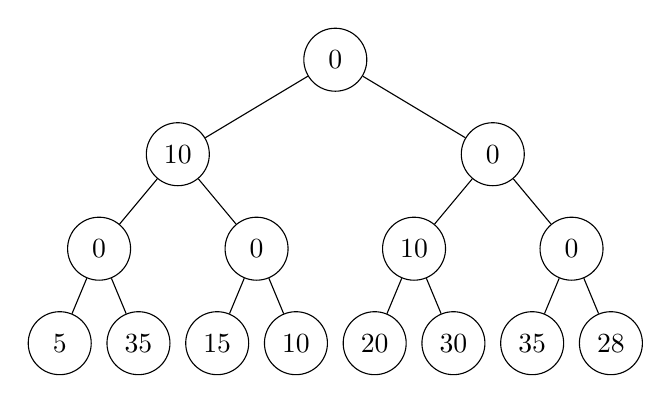
\begin{tikzpicture}[
      level distance=1.2cm,
      level 1/.style={sibling distance=4cm},
      level 2/.style={sibling distance=2cm},
      level 3/.style={sibling distance=1cm},
      every node/.style={draw,circle,minimum size=8mm,inner sep=1pt}
    ]
    
    % Root node with max value
    \node {0}
        child {node {10}
            child {node {0}
                child {node {5}}
                child {node {35}}
            }
            child {node {0}
                child {node {15}}
                child {node {10}}
            }
        }
        child {node {0}
            child {node {10}
                child {node {20}}
                child {node {30}}
            }
            child {node {0}
                child {node {35}}
                child {node {28}}
            }
        };
    
    \end{tikzpicture}
\end{center}
